Se implementó un modelo de clasificación con el propósito de predecir y comprender el comportamiento del usuario basándose en un conjunto de datos detallado y complejo.

\subsection{Preprocesamiento y Preparación de Datos}

Comenzamos con la importación de los datos desde un archivo CSV, seguida de un proceso de limpieza para asegurar la integridad de la información. En esta etapa, se filtraron registros específicos en la columna “método” y se descartaron aquellos casos donde la columna “canal” estaba vacía. Adicionalmente, las marcas temporales fueron convertidas al formato UTC para garantizar una estandarización completa a lo largo del conjunto de datos.

\subsection{Ordenamiento y Etiquetado}

Ordenamos el conjunto de datos cronológicamente por usuario y fecha de evento, para preservar la secuencia de acciones de cada usuario. Se generaron nuevas columnas que indican el siguiente método y canal utilizado por el usuario, sirviendo estas como etiquetas para el modelo de predicción que estamos diseñando.

\subsection{Identificación de Sesiones}

Calculamos el intervalo de tiempo entre eventos consecutivos para determinar el inicio de nuevas sesiones de usuario, basándonos en un umbral de tiempo preestablecido. Este umbral se seleccionó de acuerdo con la dinámica típica observada en el sitio web, considerando que una sesión representa un conjunto continuo de interacciones del usuario.

\subsection{Codificación de Categorías}

Dado que los métodos y canales son variables categóricas, los convertimos en representaciones numéricas utilizando diccionarios que asignan un valor entero único a cada categoría. Este paso es esencial para que los datos puedan ser interpretados y procesados por la red neuronal.

\subsection{Construcción de Secuencias}

Integramos las representaciones numéricas de los métodos y canales en secuencias de pares, correspondientes a cada sesión de usuario. Este enfoque nos permite modelar la secuencia de interacciones y la trayectoria de comportamiento de los usuarios.

\subsection{División de Datos}

Los datos fueron divididos en conjuntos de entrenamiento y prueba, lo que nos permite validar la capacidad del modelo de generalizar y realizar predicciones precisas en datos que no ha visto previamente.

\subsection{Construcción del Modelo}

Desarrollamos un modelo secuencial con la biblioteca Keras que incorpora capas de incrustación (Embedding) y LSTM. La capa de Embedding transforma nuestras representaciones numéricas en vectores de características densas, mientras que las capas LSTM se encargan de capturar las dependencias temporales y secuenciales presentes en los datos.


\begin{figure}[H]
    \begin{minipage}[t]{0.9\textwidth}
        \caption{Construccion del modelo de clasificación}
        \label{parquitectura_clasificación}        
    \end{minipage}

    \vspace{10pt}

    \begin{minipage}[b]{1\textwidth}
        \centering
        \includegraphics[width=\textwidth]{img/Arquitectura modelo clasificación.jpg}        
    \end{minipage}

    \begin{minipage}[t]{0.9\textwidth}
        Fuente: Elaboración propia.
    \end{minipage}
\end{figure}

\subsection{Regularización y Compilación}

Para combatir el sobreajuste, incluimos capas de Dropout después de cada capa LSTM, lo cual ayuda a que el modelo sea más robusto y menos propenso a memorizar los datos de entrenamiento. Posteriormente, compilamos el modelo con la función de pérdida de entropía cruzada categórica y el optimizador Adam para iniciar el proceso de aprendizaje.

\subsection{Entrenamiento del Modelo}

El modelo se entrenó utilizando tanto la precisión como la pérdida de validación como métricas clave para monitorear su rendimiento. Empleamos un callback de EarlyStopping que detiene el entrenamiento si no se observan mejoras en la pérdida de validación tras un cierto número de épocas. Además, este callback está configurado para restaurar los pesos del modelo al estado en que se obtuvo el mejor rendimiento en el conjunto de validación.

\subsection{Resultados del entrenamiento del modelo}

Después de completar el entrenamiento del modelo, evaluamos su rendimiento analizando las métricas de pérdida y precisión tanto en el conjunto de entrenamiento como en el de validación.

\begin{itemize}
    \item \textbf{Análisis de la Pérdida:} Los gráficos muestran que la pérdida de entrenamiento (Loss) y la pérdida de validación (Val\_Loss) disminuyen significativamente en las primeras épocas, lo que indica que el modelo está aprendiendo efectivamente de los datos. A medida que avanzan las épocas, ambas curvas de pérdida se estabilizan y convergen, lo que sugiere que el modelo ha alcanzado un punto donde realiza predicciones consistentes y fiables. La convergencia cercana de las dos líneas sugiere que el modelo no está sobreajustando, ya que la pérdida de validación no está aumentando ni divergiendo de la pérdida de entrenamiento.
    \item \textbf{Análisis de la Precisión:} En cuanto a la precisión, observamos que tanto la precisión de entrenamiento (Accuracy) como la precisión de validación (Val\_Accuracy) aumentan rápidamente y luego se estabilizan, manteniéndose muy cerca una de la otra. Esto indica un alto nivel de precisión en las predicciones del modelo y sugiere que el modelo generaliza bien a nuevos datos.
\end{itemize}

\begin{figure}[H]
    \begin{minipage}[t]{0.9\textwidth}
        \caption{Gráficos de análisis del modelo de clasificación}
        \label{gráfico_clasificación}        
    \end{minipage}

    \vspace{10pt}

    \begin{minipage}[b]{1\textwidth}
        \centering
        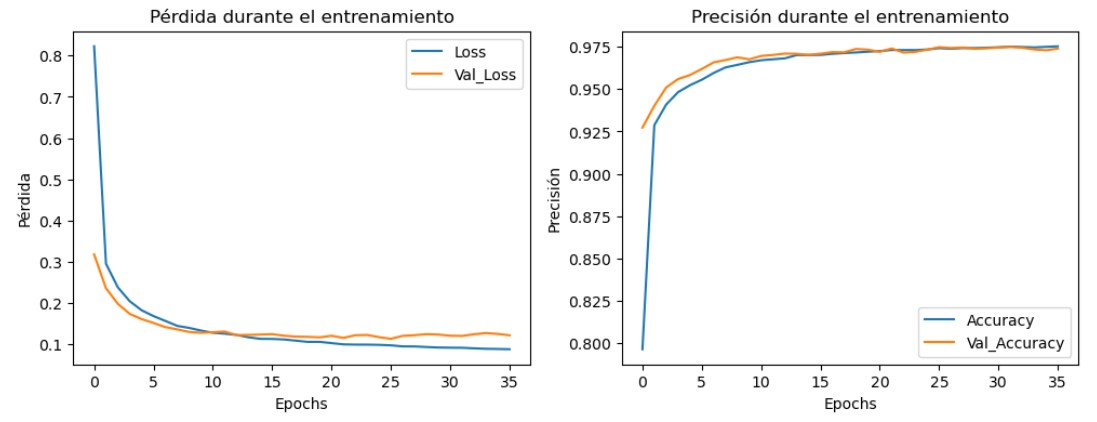
\includegraphics[width=\textwidth]{img/Gráfico modelo clasificación.jpg}        
    \end{minipage}

    \begin{minipage}[t]{0.9\textwidth}
        Fuente: Elaboración propia.
    \end{minipage}
\end{figure}

\subsection{Predicción del modelo}

Al realizar predicciones con el modelo, se utiliza una secuencia de acciones previas del usuario para predecir su siguiente acción. El modelo no solo proporciona la acción más probable sino también la confianza en su predicción, medida como una probabilidad.

Por ejemplo, si el modelo predice que el usuario seleccionará el método 'getDetails()' a continuación, también proporcionará la probabilidad asociada con esa predicción, por ejemplo, un 95\%. 

Otro ejemplo es con el método 'getAccounts()' el cual predice lo siguiente: El siguiente método predicho es: getSSContributionsCertificate() con una probabilidad del 78.76\%